\documentclass[conference]{IEEEtran}
\usepackage{cite}
\usepackage{amsmath,amssymb,amsfonts}
\usepackage{algorithmic}
\usepackage{graphicx}
\usepackage{textcomp}
\usepackage{xcolor}

\usepackage{pgfplots}
\pgfplotsset{compat=1.17}
\pgfplotscreateplotcyclelist{my color list}{black,red,blue,brown,teal,orange,violet,cyan,green!70!black,magenta,gray}

\usepgfplotslibrary{fillbetween}

\usepackage{listings}

\definecolor{codegreen}{rgb}{0,0.6,0}
\definecolor{codegray}{rgb}{0.5,0.5,0.5}
\definecolor{codepurple}{rgb}{0.58,0,0.82}
\definecolor{backcolour}{rgb}{0.95,0.95,0.92}

\lstdefinestyle{mystyle}{
    backgroundcolor=\color{backcolour},   
    commentstyle=\color{codegreen},
    keywordstyle=\color{magenta},
    numberstyle=\tiny\color{codegray},
    stringstyle=\color{codepurple},
    basicstyle=\ttfamily\footnotesize,
    breakatwhitespace=false,         
    breaklines=true,                 
    captionpos=b,                    
    keepspaces=true,                 
    numbers=left,                    
    numbersep=5pt,                  
    showspaces=false,                
    showstringspaces=false,
    showtabs=false,                  
    tabsize=2
}
\lstset{style=mystyle}

\def\BibTeX{{\rm B\kern-.05em{\sc i\kern-.025em b}\kern-.08em
    T\kern-.1667em\lower.7ex\hbox{E}\kern-.125emX}}

\begin{document}

\begin{titlepage}

    % You need to edit the details here

    \begin{center}
        {\LARGE University of Sheffield}\\[1.5cm]
        \linespread{1.2}\huge {\bfseries Assignment 2: Reinforcement Learning}\\[1.5cm]
        \linespread{1}
        
\includegraphics[width=5cm]{images/tuoslogo.png}\\[1cm]
        {\large COM3240 Adaptive Intelligence (SPRING 2020--21)}\\[1cm]
        {\Large Boxuan Shan}\\[6cm]
        \large Department of Computer Science\\[1cm]
        \today
    \end{center}

\end{titlepage}

\title{Reinforcement Learning}

\author{\IEEEauthorblockN{Boxuan Shan}
\IEEEauthorblockA{\textit{Department of Computer Science} \\
\textit{The University of Sheffield}\\
Sheffield, UK \\
bshan3@sheffield.ac.uk}
}

\maketitle

% Enable pagenumber
\thispagestyle{plain}
\pagestyle{plain}

\begin{abstract}
    Reinforcement Learning is an important branch of machine learning, which emphasis on how to act based on the environment and current state of the agent to maximise the expected rewards. In this report, a homing problem has been designed. Based on this problem, the role of SARSA, \({\epsilon}\)-Greedy, and Eligibility Trace in reinforcement learning will then be explored, as well as the effect of hyperparameters on model performance. Then, the method of rendering the preferred direction in the homing problem will also be discussed. Finally, a discussion will also be conducted on how reinforcement models can be applied to problems with larger scale. As well as the performance of the model when adding obstacles to the existing environment to complicate the problem.
\end{abstract}

\begin{IEEEkeywords}
    Reinforcement Learning, Homing problem, SARSA, Eligibility trace
\end{IEEEkeywords}

\section{Introduction}

The main idea of reinforcement learning~\cite{richard2018rl} is to emphasise how to act based on the environment and the current state in order to maximise the expected rewards. In contrast to supervised learning, this approach does not require comprehensive knowledge of the environment or a labelled dataset to be provided in advance, only the definition of reward and punishment of different behaviours in the environment is required. Therefore this is often used in situations where the environment and decision trees is complex while the knowledge of it is limited. In this report, a homing problem has been designed. A robot is placed in a 10\({\times}\)10 space and trained to find a goal by reinforcement learning. In this case, the 10\({\times}\)10 space is the environment, and the robot is the agent in reinforcement learning, whose position is the current state. This problem will be used to experiment with the \(SARSA\) algorithm, the \({\epsilon}\)-Greedy policy and the Eligibility Trace in reinforcement learning. Then, obstacles will be added to the space in order to test the performance of reinforcement learning.

\section{Methods}

In this experiment, a neural network will use to model Q-values. In this case, the input to the neural network is the current state of the agent, which is the encoded current position of the robot. The output of the neural network represents the predicted reward Q-values for performing different actions from the current state, and the weights in the neural network will be updated during the training process. Ideally, when the training converges, the predicted rewards are expected to be the same as the actual reward.

\subsection{\(SARSA\)}

In this experiment, the \(SARSA\)~\cite{richard2018sarsa} algorithm is used to update the weights of the neural network, and thus the Q-values. This is a training method that takes future rewards into account. Its mathematical expression for the Q-value update is as follows.

\begin{equation}
    \Delta Q(s,a)= \eta \left[r-\left(Q(s,a)-\gamma Q(s^\prime,a^\prime)\right)\right]
\end{equation}

where \(Q(s,a)\) this the predicted expected reward of taking action \(a\) in state \(s\), \(r\) is the corresponding true expected reward. \(Q(s^\prime,a^\prime)\) is the predicted expected reward by the next action performed by the policy after \(Q(s,a)\). In this case, the policy is to perform the action with maxmimum predicted expected reward.  \({\gamma}\) is a discount factor for future rewards to weight the effect of it. \({\eta}\) is the learning rate.

Therefore, the update of the weights of the neural network can be obtained as follows.

\begin{eqnarray}
    \delta &=& r-\left(Q(s,a)-\gamma Q(s^\prime,a^\prime)\right) \\
    \Delta w_{ij} &=& \eta \delta y_i x_j
\end{eqnarray}

where \({\delta}\) is the update factor, \(x\) is the encoded current status, \(y\) is the desired output. \(\Delta w_{ij}\) is the changes in weight for \(y_i\) and \(x_j\).

\subsection{\({\epsilon}\)-Greedy}

\(SARSA\) is an on-policy update approach. If assuming that the policy is simply designed to always choose the action with the largest predicted reward as the next step, the model will find a path to the goal eventually. However, in this way, if the model finds a path that leads to the goal, it will keep following that path in subsequent trails to receive rewards. That path is then continuously reinforced and thus the ability to explore other paths is lost. This is not expected, as it is possible to fall into a local optimum and thus not find the globally optimal path. The \({\epsilon}\)-Greedy algorithm~\cite{richard2018sarsa} is therefore used to address this problem. Instead of following the action with maxmimum predicted rewards constantly, it randomly chooses the next action with the probability of \({\epsilon}\). At this point, the model will be forced to explore more space.

\subsection{Eligibility Trace}

Since \(SARSA\) will only update two adjacent states at a time, when the model attempts to reinforce a path, it will update step by step from the source of the reward, which is the goal, towards the starting point. Since our model does not have the ability to trace paths, it will only update the path it wants to reinforce by one unit per trials towards the starting point. This means that multiple trials are required to update the complete entire path. Therefore, Eligibility Trace will be introduced to make a trace of the path from the starting point to the current position. In this way, the Q-values of the entire path can be updated with a single update when the agent is rewarded, which is expected to speed up the training of the model. This approach is also refer as \(SARSA(\lambda)\)~\cite{richard2018sarsalambda}.

In this case, the mathematical expression for the weight update becomes today
\begin{eqnarray}
    e_{ij} = \gamma \lambda e_{ij} + y_i x_i \\
    \Delta w_{ij} = \eta \delta e_{ij}
\end{eqnarray}

where \(e_{ij}\) is the variable for tracing. The  \(e_{ij}\) corresponding to the action being performed will be enhanced and the rest will decay at each update, where \({\lambda}\) is the decay factor. \(\Delta w_{ij}\) is the update for weights.

\section{Results and Discussion}

In the experiments, the maximum number of steps is set to 50, and when the number of steps is exceeded, the trail is terminated with a penalty factor of -1. When the agent exceeds the space boundary or hits an obstacle, a penalty factor of -0.1 is given and the agent's movement is ignored and restored to the previous state. The goal location will be randomly generated for each run, and the starting point of each trail will be randomly generated as well. 

\subsection{Exploration}

In this section, we will experiment with the effect of the \({\epsilon}\)-Greedy policy on the explorability of the model. The \({\epsilon}\)-Greedy policy is used as the decision policy together with the \(SARSA\) algorithm for Q-value updates. When \({\epsilon}\) is set to 0, it is a full greedy policy and the model will always choose the current optimal action without exploring any new space. When \({\epsilon}\) is set to 1, it is a completely randomized policy and the model will be difficult to converge as the agent will explore a lot of space that not in the optimal path. Neither of these is expected, therefore a reasonable \({\epsilon}\) should be between 0 and 1. In the experiments, we set the learning rate \({\eta}\) to 0.3 and the discount factor \({\gamma}\) to 0.9. A total of 100 run were performed, with 2000 trials performed each time, and the mean value was calculated afterwards. The training curve is shown in Figure~\ref{fig:exploration}.

\begin{figure}[!ht]
    \centering
    \begin{tikzpicture}[scale = 0.8]
        \begin{axis}[
            title={},
            xlabel={Trials},
            ylabel={Average Steps},
            legend pos=north east,
            grid=both,
            grid style=dashed,
        ]
            \addplot+ [mark=none, opacity=0.6, color=black] table[x=trail,y=mean, col sep=comma] {data/exploration/eps-0.0.csv};
            \addlegendentry{\(\epsilon=0.0\)}
            \addplot+ [mark=none, opacity=0.6, color=red] table[x=trail,y=mean, col sep=comma] {data/exploration/eps-0.1.csv};
            \addlegendentry{\(\epsilon=0.1\)}
            \addplot+ [mark=none, opacity=0.6, color=green] table[x=trail,y=mean, col sep=comma] {data/exploration/eps-0.5.csv};
            \addlegendentry{\(\epsilon=0.5\)}
            \addplot+ [mark=none, opacity=0.6, color=blue] table[x=trail,y=mean, col sep=comma] {data/exploration/eps-0.7.csv};
            \addlegendentry{\(\epsilon=0.7\)}
        \end{axis}
    \end{tikzpicture}
    \caption{Average Steps vs Trials with different \({\epsilon}\)}\label{fig:exploration}
\end{figure}

From the figure, it is clear that as \({\epsilon}\) increases, the average number of steps decreases slower. This may be caused by the model's tendency to explore more spaces and paths during the training process. Through this experiment, it was not found that \({\epsilon}\)-Greedy could significantly improve the model performance in our scenario. This may be due to the fact that our problem is too simple, where the number of states and actions is not very large, and therefore the entire space can be explored without explicitly exploring policies and algorithms. However, for more complex problems, exploration may be necessary.

\subsection{Optimal Hyperparameters}

In this section, the optimal learning rate \({\eta}\), discount factor \({\gamma}\) and exploration factor \({\epsilon}\) will be experimented with. In the following experiments, each set of parameters was run 100 times, with 2000 trails performed each time, and then the averages over 100 runs were calculated. In addition, the average number of extra steps over the optimal path for each set of hyperparameters was also be calculated, where the distance of the optimal path will be represented by the Manhattan distance. Then the standard deviation of extra steps over runs has been calculated.

\subsubsection{Optimal Learning Rate}

In this experiment, the discount factor \({\gamma}\) was set to a fixed value of 0.9 and the exploration factor \({\epsilon}\) was set to a fixed value of 0.0. The effect of different learning rates \({\eta}\) on the performance of the model was then experimented with. The results are shown in Figure~\ref{fig:eta} and Figure~\ref{fig:etaExtra}.

\begin{figure}[!ht]
    \centering
    \begin{tikzpicture}[scale = 0.8]
        \begin{axis}[
            title={},
            xlabel={Trials},
            ylabel={Average Steps},
            legend pos=north east,
            grid=both,
            grid style=dashed,
        ]

            \addplot+ [mark=none, opacity=0.6, color=red] table[x=trail,y=mean, col sep=comma] {data/optimal/lr/0.1.csv};
            \addlegendentry{\(\eta=0.1\)}
            \addplot+ [mark=none, opacity=0.6, color=green] table[x=trail,y=mean, col sep=comma] {data/optimal/lr/0.3.csv};
            \addlegendentry{\(\eta=0.3\)}
            \addplot+ [mark=none, opacity=0.6, color=blue] table[x=trail,y=mean, col sep=comma] {data/optimal/lr/0.5.csv};
            \addlegendentry{\(\eta=0.5\)}
            \addplot+ [mark=none, opacity=0.6, color=cyan] table[x=trail,y=mean, col sep=comma] {data/optimal/lr/0.7.csv};
            \addlegendentry{\(\eta=0.7\)}
            \addplot+ [mark=none, opacity=0.6, color=magenta] table[x=trail,y=mean, col sep=comma] {data/optimal/lr/0.9.csv};
            \addlegendentry{\(\eta=0.9\)}
        \end{axis}
    \end{tikzpicture}
    \caption{Average Steps vs Trials with different learning rate \({\eta}\)}\label{fig:eta}
\end{figure}

\begin{figure}[!ht]
    \centering
    \begin{tikzpicture}[scale = 0.8]
        \begin{axis}[
            title={},
            xlabel={Trials},
            ylabel={Average Extra Steps},
            legend pos=north east,
            grid=both,
            grid style=dashed,
        ]
            \addplot+ [mark=none, opacity=0.6, color=black, error bars/.cd, y fixed, y dir=both, y explicit] table[x=eta, y=mean, y error=std, col sep=comma] {data/extra_step/eta.csv};
        \end{axis}
    \end{tikzpicture}
    \caption{Average Extra Steps vs different learning rate \({\eta}\)}\label{fig:etaExtra}
\end{figure}

The figure shows that when the learning rate \({\eta}\) is set to 0.9, the model achieves optimal performance at 2000 trails. If the learning rate is too low, the convergence rate is too slow and more trails are needed to achieve its best performance.

\subsubsection{Optimal Discount Factor}

In this experiment, the learning rate \({\eta}\) was set to the optimal value of 0.9 and the exploration factor \({\epsilon}\)  was set to a fixed value of 0.0. The effect of different discount factor \({\gamma}\) on the performance of the model was then experimented with. The results are shown in Figure~\ref{fig:gamma} and Figure~\ref{fig:gammaExtra}.

\begin{figure}[!ht]
    \centering
    \begin{tikzpicture}[scale = 0.8]
        \begin{axis}[
            title={},
            xlabel={Trials},
            ylabel={Average Steps},
            legend pos=north east,
            grid=both,
            grid style=dashed,
        ]
            \addplot+ [mark=none, opacity=0.6, color=red] table[x=trail,y=mean, col sep=comma] {data/optimal/discount/0.7.csv};
            \addlegendentry{\(\gamma=0.7\)}
            \addplot+ [mark=none, opacity=0.6, color=green] table[x=trail,y=mean, col sep=comma] {data/optimal/discount/0.8.csv};
            \addlegendentry{\(\gamma=0.8\)}
            \addplot+ [mark=none, opacity=0.6, color=blue] table[x=trail,y=mean, col sep=comma] {data/optimal/discount/0.9.csv};
            \addlegendentry{\(\gamma=0.9\)}
            \addplot+ [mark=none, opacity=0.6, color=cyan] table[x=trail,y=mean, col sep=comma] {data/optimal/discount/1.0.csv};
            \addlegendentry{\(\gamma=1.0\)}
        \end{axis}
    \end{tikzpicture}
    \caption{Average Steps vs Trials with different discount factor \({\gamma}\)}\label{fig:gamma}
\end{figure}

\begin{figure}[!ht]
    \centering
    \begin{tikzpicture}[scale = 0.8]
        \begin{axis}[
            title={},
            xlabel={Trials},
            ylabel={Average Extra Steps},
            legend pos=north east,
            grid=both,
            grid style=dashed,
        ]
            \addplot+ [mark=none, opacity=0.6, color=black, error bars/.cd, y fixed, y dir=both, y explicit] table[x=eta, y=mean, y error=std, col sep=comma] {data/extra_step/gamma.csv};
        \end{axis}
    \end{tikzpicture}
    \caption{Average Extra Steps vs different discount factor \({\gamma}\)}\label{fig:gammaExtra}
\end{figure}

As shown in the figure, when the discount factor \({\gamma}\) is 0.9, the model has the best performance within 2000 trails. When \({\gamma}\) is smaller (e.g. 0.8, 0.7), the influence of future rewards on the decision is lower, which slows down the convergence of the model in the current scenario. When \({\gamma}\) is higher (e.g., 1.0), the influence of future rewards on the decision is higher, and the model's performance is reduced in the current scenario.

\subsubsection{Optimal Discount Factor}

In this experiment, the learning rate \({\eta}\) was set to the optimal value of 0.9 and the discount factor \({\gamma}\)  was set to the optimal value of 0.9. The effect of different exploration factor \({\epsilon}\) on the performance of the model was then experimented with. The results are shown in Figure~\ref{fig:epsilon} and Figure~\ref{fig:epsilonExtra}.

\begin{figure}[!ht]
    \centering
    \begin{tikzpicture}[scale = 0.8]
        \begin{axis}[
            title={},
            xlabel={Trials},
            ylabel={Average Steps},
            ymax=20,
            legend pos=north east,
            grid=both,
            grid style=dashed,
        ]
            \addplot+ [mark=none, opacity=0.6, color=red] table[x=trail,y=mean, col sep=comma] {data/optimal/exploration/0.0.csv};
            \addlegendentry{\(\epsilon=0.0\)}
            \addplot+ [mark=none, opacity=0.6, color=green] table[x=trail,y=mean, col sep=comma] {data/optimal/exploration/0.05.csv};
            \addlegendentry{\(\epsilon=0.05\)}
            \addplot+ [mark=none, opacity=0.6, color=blue] table[x=trail,y=mean, col sep=comma] {data/optimal/exploration/0.1.csv};
            \addlegendentry{\(\epsilon=0.1\)}
            \addplot+ [mark=none, opacity=0.6, color=cyan] table[x=trail,y=mean, col sep=comma] {data/optimal/exploration/0.2.csv};
            \addlegendentry{\(\epsilon=0.2\)}
            
        \end{axis}
    \end{tikzpicture}
    \caption{Average Steps vs Trials with different exploration factor \({\epsilon}\)}\label{fig:epsilon}
\end{figure}

\begin{figure}[!ht]
    \centering
    \begin{tikzpicture}[scale = 0.8]
        \begin{axis}[
            title={},
            xlabel={Trials},
            ylabel={Average Extra Steps},
            legend pos=north east,
            grid=both,
            grid style=dashed,
        ]
            \addplot+ [mark=none, opacity=0.6, color=black, error bars/.cd, y fixed, y dir=both, y explicit] table[x=eta, y=mean, y error=std, col sep=comma] {data/extra_step/epsilon.csv};
        \end{axis}
    \end{tikzpicture}
    \caption{Average Extra Steps vs different exploration factor \({\epsilon}\)}\label{fig:epsilonExtra}
\end{figure}

As shown in the figure, the model has optimal performance when the exploration factor \({\epsilon}\) is 0. 
This is equivalent to a full on-policy algorithm, where the model can explore new spaces and paths reasonably well, while not causing a lot of disturbance to the best paths currently explored. When \({\epsilon}\) increases, the model will attempt to explore the space beyond the current optimal path, thus potentially discovering paths that are better than the current optimal path. However, in our problem, probably because the problem is too simple and the number of states and their actions are not very large, explicitly increasing the exploration capability does not significantly improve the model performance.

\subsection{Eligibility Trace}

\(SARSA(\lambda)\) is the \(SARSA\) that introduces the Eligibility Trace mechanism, which updates the entire path at once after the reward is obtained. Therefore \(SARSA(\lambda)\) is expected to have a faster learning speed than \(SARSA\). For the trace decay factor \({\lambda}\), a larger value means that the weaker the decay of the path in the trace, where the update has a stronger effect on previous steps in the trace.

In this experiment, the learning rate \({\eta}\) was set to the optimal value of 0.9, the discount factor \({\gamma}\) was set to the optimal value of 0.9 and the exploration factor \({\epsilon}\) was set to the optimal value of 0.0. The effect of trace decay factor \({\lambda}\) on the performance of the model was then experimented with. The training curve is shown in Figure~\ref{fig:trace}.

\begin{figure}[!ht]
    \centering
    \begin{tikzpicture}[scale = 0.8]
        \begin{axis}[
            title={},
            xlabel={Trials},
            ylabel={Average Steps},
            ymax=20,
            legend pos=north east,
            grid=both,
            grid style=dashed,
        ]
            \addplot+ [mark=none, opacity=0.6, color=red] table[x=trail,y=mean, col sep=comma] {data/lambda/0.9.csv};
            \addlegendentry{\(SARSA(\lambda)\), \({\lambda}=0.9\)}

            \addplot+ [mark=none, opacity=0.6, color=green] table[x=trail,y=mean, col sep=comma] {data/lambda/0.7.csv};
            \addlegendentry{\(SARSA(\lambda)\), \({\lambda}=0.7\)}

            \addplot+ [mark=none, opacity=0.6, color=blue] table[x=trail,y=mean, col sep=comma] {data/lambda/0.3.csv};
            \addlegendentry{\(SARSA(\lambda)\), \({\lambda}=0.3\)}

            \addplot+ [mark=none, opacity=0.6, color=cyan] table[x=trail,y=mean, col sep=comma] {data/optimal/exploration/0.0.csv};
            \addlegendentry{\(SARSA\)}

        \end{axis}
    \end{tikzpicture}
    \caption{Average Steps vs Trials with different trace decay factor \({\lambda}\)}\label{fig:trace}
\end{figure}

The figure shows that when the value of \({\lambda}\) is large (e.g., 0.9) the model has a faster learning speed. However, it will stop learning sooner and the final converged optimal path is not as good as the \(SARSA\) algorithm. As \({\lambda}\) becomes progressively smaller, its learning curve gradually converges to that of the \(SARSA\) algorithm.

\subsection{Preferred Direction}

For each position in the 10\({\times}\)10 space, there is a corresponding state representation. Therefore, for each position, we can obtain its preferred action, for which we use arrows to represent the four different actions. An example is shown in the Figure~\ref{fig:direc}.

\begin{figure}[!ht]
    \centering
    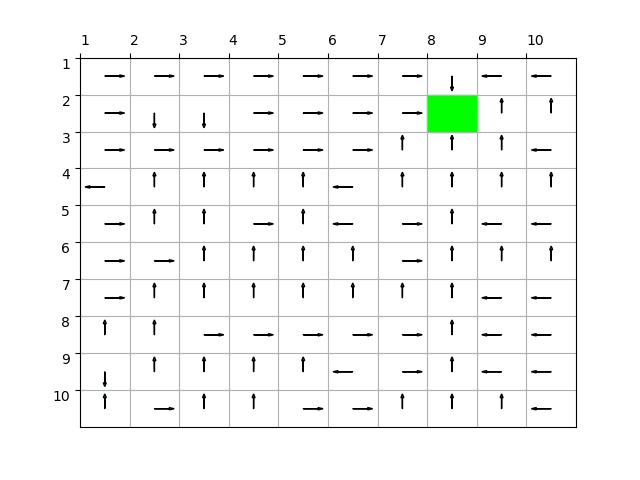
\includegraphics[width=.45\textwidth]{figures/preferred_direc/0.png}
    \caption{Preferred Direction Map}\label{fig:direc}
\end{figure}

where the green box shows the location of the goal. The figure shows that, after training, for the most of the locations, the preferred action tends to point in a direction that is approaching the goal. This indicates that our model tends to navigate the agent to move towards the goal.

\subsection{Large scale problem}

As the scale of the problem becomes larger, the depth of the decision tree will increase and it will be more difficult for the agent to explore all the paths directly. Therefore, the exploration will become more important. In this case, the \({\epsilon}\) value of \({\epsilon}\)-Greedy can be increased appropriately to force the agent to explore more spaces and paths. 

Furthermore, as the number of states increases, the input layers of the neural network will become larger and thus the computational complexity will increase significantly. To address this problem, a layered approach can be adopted, where the entire space is divided into multiple sub-regions. Firstly, a decision model is built to make decisions in a large space, in terms of sub-regions. Then separate decision models are built within each sub-region. At this point, only the macro inter-regional decisions and the micro decisions within the corresponding regions need to be considered. Decisions for the remaining sub-regions need not be considered. This approach significantly reduces the computational complexity.

\subsection{Complex problem}

In this section, obstacles are added to the space to make the problem more complex and the model is trained on this basis. In this experiment, the learning rate \({\eta}\) was set to the optimal value of 0.9, the discount factor \({\gamma}\) was set to the optimal value of 0.9 and the \({\lambda}\) for eligibility trace is set to 0.3. Since this problem is relatively complex, the exploration factor \({\epsilon}\) is adjusted slightly upwards to 0.2. An example result of preferred direction for each location is shown in Figure~\ref{fig:complex}.

\begin{figure}[!ht]
    \centering
    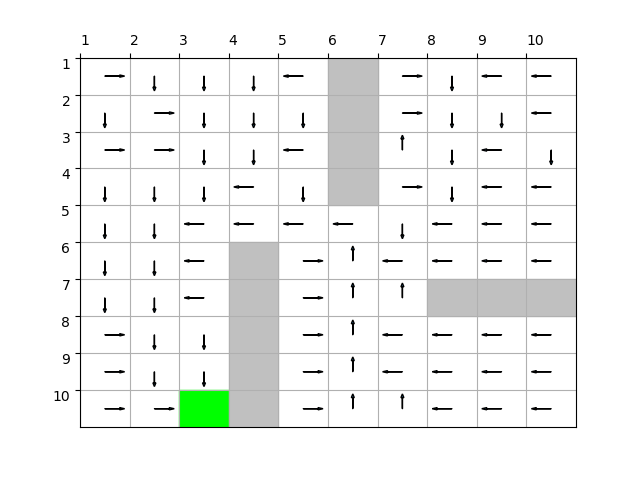
\includegraphics[width=.45\textwidth]{figures/complex_direc/5.png}
    \caption{Preferred Direction Map with obstacles}\label{fig:complex}
\end{figure}
where the the green block represents the goal, grey blocks represent the obstacle and arrows represent the preferred direction of positions.

The figure shows that our model can correctly navigate the agent to the goal, that is, no matter which position it starts from, by following the direction of arrows, it will eventually reach the goal. At the same time, it can be noted that the direction of the arrow will guide the agent to avoid obstacles and thus avoid penalties.

\bibliographystyle{IEEEtran}
\bibliography{bibliography}

\onecolumn
\appendices{}

\section{Implementation of \({\epsilon}\)-Greedy policy}

\begin{lstlisting}[language=Python]
greedy = (np.random.rand() > eps)               # 1--->greedy action 0--->non-greedy action
if greedy:
    action = np.argmax(q_s)                     # pick best action
else:
    action = np.random.randint(N_actions)       # pick random action

\end{lstlisting}

\section{Implementation of rewarding}

\begin{lstlisting}[language=Python]
r = 0
# put the robot back in grid if it goes out. Consider also the option to give a negative reward
if state_new[0] < 0:
    state_new[0] = 0
    r = PENALIZE_EDGE
if state_new[0] >= M:
    state_new[0] = M-1
    r = PENALIZE_EDGE
if state_new[1] < 0:
    state_new[1] = 0
    r = PENALIZE_EDGE
if state_new[1] >= N:
    state_new[1] = N-1
    r = PENALIZE_EDGE

# walls hittest
if (state_new[0], state_new[1]) in walls:
    state_new = state
    r = PENALIZE_WALL

\end{lstlisting}

\section{Implementation of \(SARSA\) and \(SARSA(\lambda)\) weight updating}

\begin{lstlisting}[language=Python]
if step > 1:
    delta = r_old - q_sa_old + gamma * q_s[action]
    if lam > 0:
        dw = learning_rate * delta * e
    else:
        dw = learning_rate * delta * output_old.dot(input_old.T)
        
    weights += dw

if lam > 0:
    e = gamma * lam * e
    e[action, s_index] = e[action, s_index] + 1

\end{lstlisting}

\section{Implementation of weight updating at final step}

\begin{lstlisting}[language=Python]
if s_index == s_end:
    # reward reached
    r_old = REWARD
elif step == n_steps:
    # steps exceeded
    r_old = PENALIZE_EXCEEDED
# update weights
delta = r_old - q_sa_old
if lam > 0:
    dw = learning_rate * delta * e
else:
    dw = learning_rate * delta * output_old.dot(input_old.T)
weights += dw

\end{lstlisting}

\section{Implementation of preferred direction drawing}

\begin{lstlisting}[language=Python]
def draw_preferred_direc(weights, goal, walls, save_path=None):
    """draw preferred directions for each position in the playground.

    Args:
        weights: weight of the neural network
        goal: goal position
        walls: walls position
        save_path: path to save the image, None for show in window
    """
    plt.figure()
    
    plt.xlim((1, 1+M))
    plt.ylim((1, 1+N))
    plt.gca().xaxis.set_ticks_position('top')
    plt.gca().invert_yaxis()
    plt.xticks(np.arange(1, 1+M, step=1), ha='left')
    plt.yticks(np.arange(1, 1+N, step=1), va='top')
    plt.grid()

    for x in range(M):
        for y in range(N):
            if x == goal[0] and y == goal[1]:
                continue
            if (x, y) in walls:
                continue

            s_test = np.ravel_multi_index(np.array([x, y]),dims=(M,N),order='F')
            input_vector = states_matrix[:,s_test].reshape(N_states,1)
            Q = 1 / ( 1 + np.exp( - weights.dot(input_vector)))
            action = np.argmax(Q)

            r_c = action_row_change[action]
            c_c = action_col_change[action]
            
            plt.arrow(x+1.5, y+1.5, c_c * 0.3, r_c * 0.3, head_width=0.06, head_length=0.1)

    goal_rect = patches.Rectangle([goal[0]+1, goal[1]+1], 1, 1, linewidth=1, edgecolor='lime', facecolor='lime')
    plt.gca().add_patch(goal_rect)

    for wall in walls:
        wall_rect = patches.Rectangle([wall[0]+1, wall[1]+1], 1, 1, linewidth=1, edgecolor='silver', facecolor='silver')
        plt.gca().add_patch(wall_rect)

    if save_path:
        plt.savefig(save_path)
        plt.close()
    else:
        plt.show()

\end{lstlisting}

\end{document}
